% v9.5 appendix (2026-10-25): analyses numbered E1--E13; E2 and E9 figures removed (values in tab:ladder and tab:fill).
\clearpage
\appendix
\section{Supplementary exploratory figures}

All figures in this appendix come from the exploratory analyses described in Section~\ref{sec:posthoc}. They use S12-only checkpoint selection unless stated otherwise, show means over three seeds, and use the same independent test set as the main results. Source code is in \texttt{posthoc/} and outputs are in \texttt{experiments/posthoc/} of the supplementary material; script and folder names there use the original proposal numbers, and the supplementary README maps them to E1--E13.

\begin{figure}[htbp]
\centering
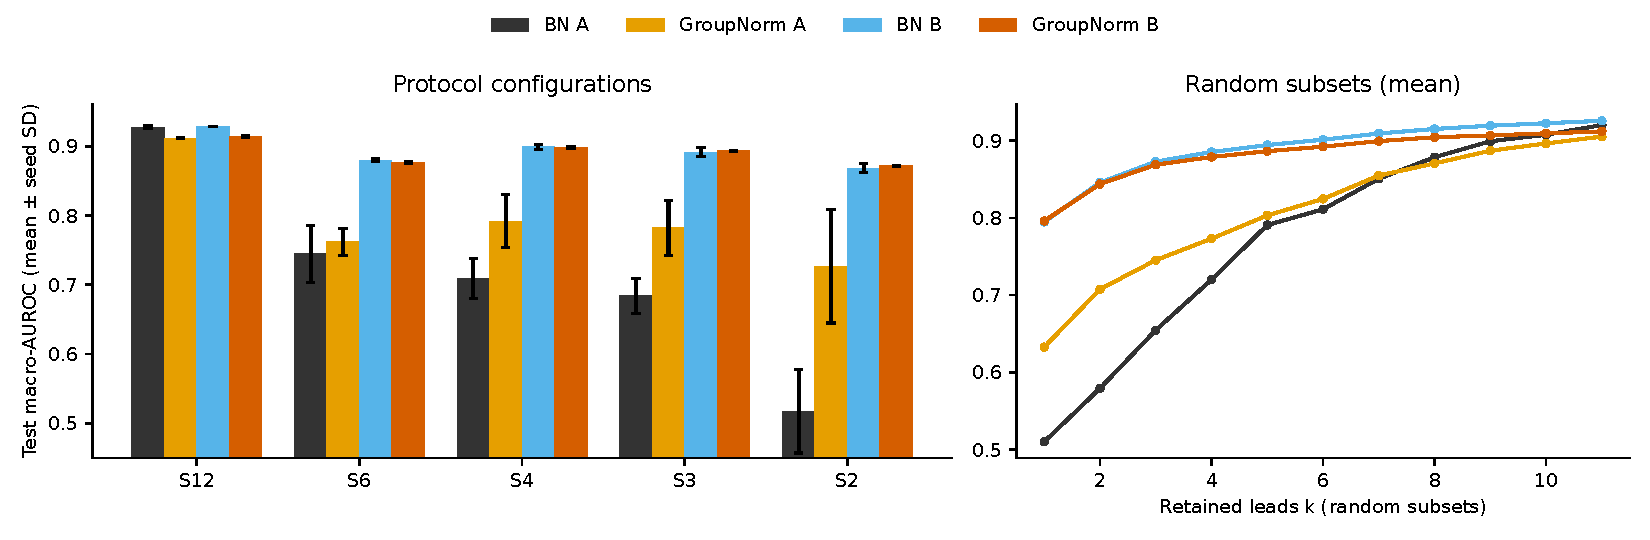
\includegraphics[width=\linewidth]{figures/e8_normalization_ablation.pdf}
\caption{E7: BatchNorm versus GroupNorm(8) for both arms. Left: protocol configurations (mean $\pm$ seed SD). Right: mean over random subsets by retained count. GroupNorm improves complete-input training under missing leads, stays below masked training, and costs about 0.015 complete-input AUROC without re-tuning.}
\label{fig:e8}
\end{figure}

\begin{figure}[htbp]
\centering
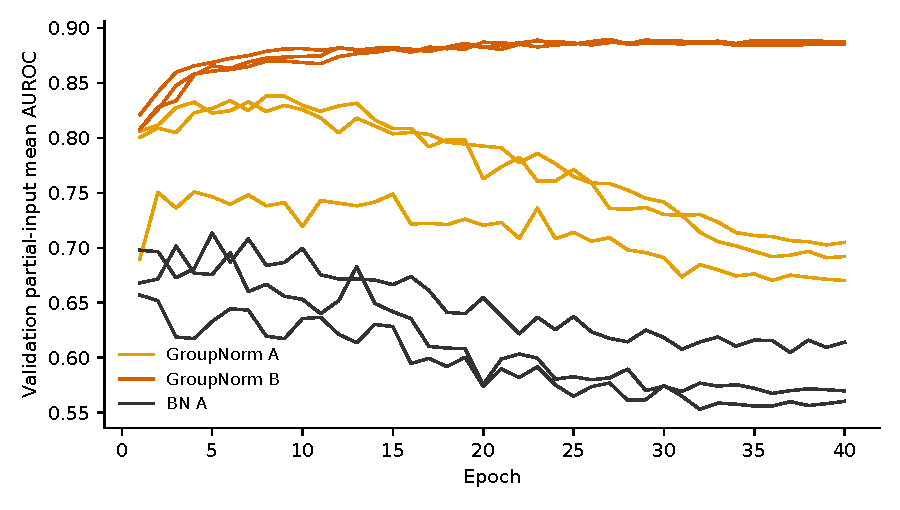
\includegraphics[width=0.7\linewidth]{figures/e8_training_dynamics.pdf}
\caption{E7: validation partial-input mean AUROC by epoch. GroupNorm A starts higher than BatchNorm A and also declines with training, which indicates reliance on the complete lead set beyond normalization statistics.}
\label{fig:e8dyn}
\end{figure}

\begin{figure}[htbp]
\centering
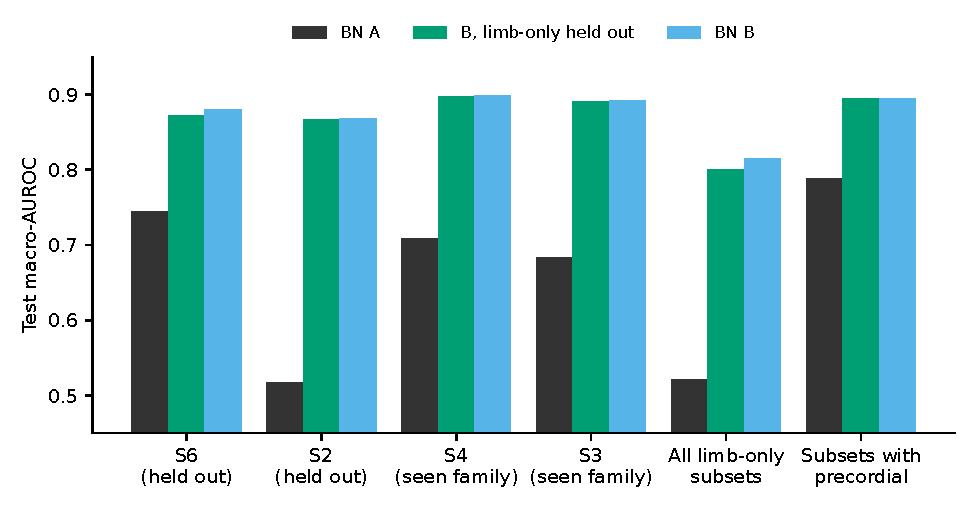
\includegraphics[width=0.8\linewidth]{figures/e9_heldout_limb_family.pdf}
\caption{E8: masked training with every limb-only partial input withheld (HO B), compared with S12-selected A and B (``BN A'' and ``BN B''). S6 and S2 are unseen in training; S4 and S3 belong to a seen family. The last two groups average over all limb-only conditions evaluated in E5 (21 conditions, 15 distinct subsets) and all other partial-input conditions (199), among the 220 partial-input conditions evaluated in E5 (4 protocol sets, 12 single-lead sets and 204 random subsets).}
\label{fig:e9}
\end{figure}

\begin{figure}[htbp]
\centering
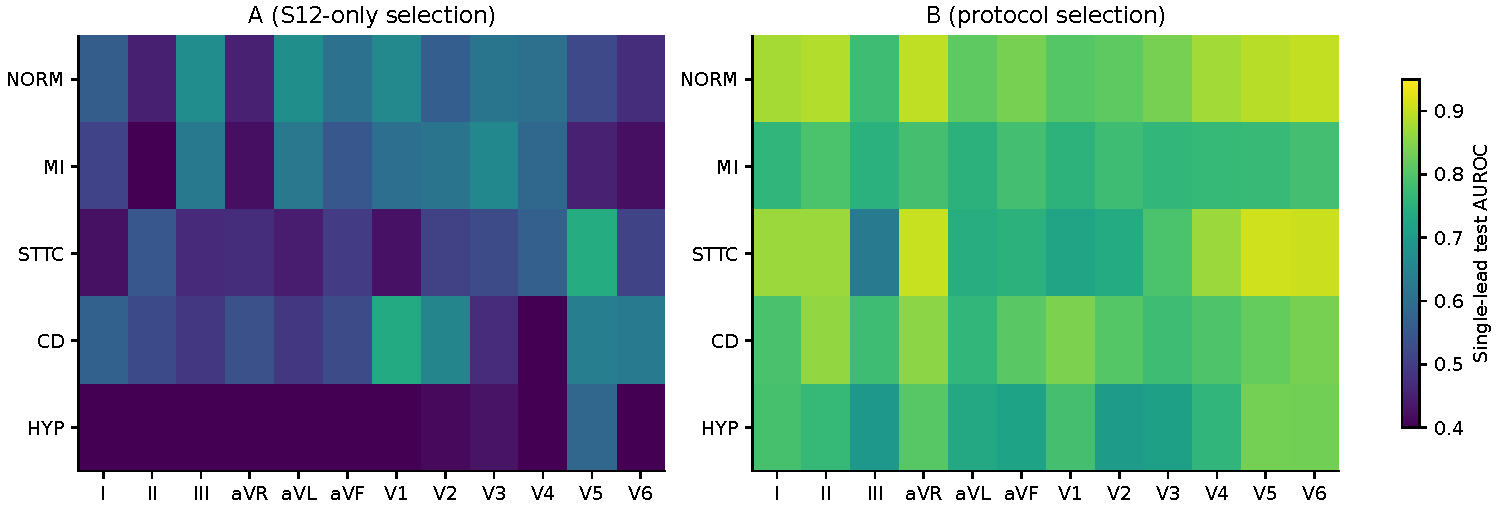
\includegraphics[width=\linewidth]{figures/e6_single_lead_per_label.pdf}
\caption{E5: per-label test AUROC with a single retained lead, for complete-input training (A, S12-only selection) and masked training (B, protocol selection).}
\label{fig:e6label}
\end{figure}

\clearpage
\section{Data audit and class examples}
\label{app:data}

The following checks cover the computational reliability of the data pipeline.
\begin{itemize}
\item \textbf{Independent reader.} On a 100-record training pilot sample, an independently implemented format-16 reader matched WFDB exactly over 1.2 million float32 values.
\item \textbf{Re-decoding.} 40 development recordings (20 + 20 sampled evenly from the training and validation splits) and 30 test recordings were re-decoded from the raw WFDB files and re-standardized with the same reader and normalization code; all values matched the stored arrays. These recomputations test consistency of the same code.
\item \textbf{Hashes and alignment.} The hashes of all original files and prepared arrays were recorded, and labels were checked against record order for every split.
\item \textbf{Normalization.} Means and variances were accumulated in float64 and stored as float32. The 0.000001\,mV floor on the standard deviation was never triggered.
\item \textbf{Test timing.} The six checkpoint hashes were fixed at 2026-10-22 18:55 UTC, and the pipeline first parsed fold-10 diagnostic codes at 20:20 UTC the same day.
\end{itemize}

\begin{figure}[htbp]
\centering
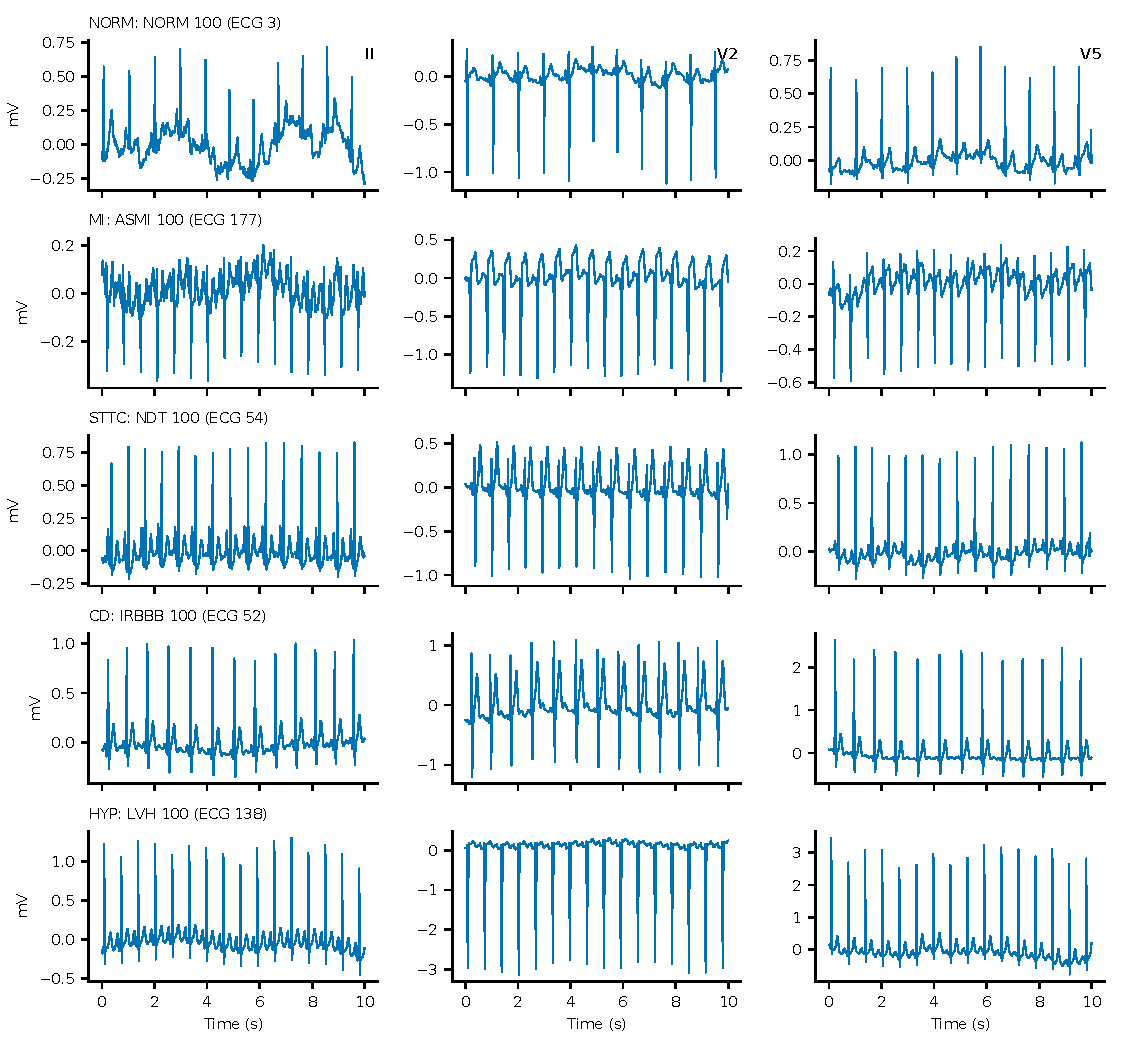
\includegraphics[width=\linewidth]{figures/appendix_class_examples.pdf}
\caption{Leads II, V2 and V5 (in mV) of one training record per diagnostic superclass. Records were selected from metadata alone: exactly one superclass, every diagnostic statement at likelihood 100, human-validated labels, age at least 18 and no PTB-XL signal-quality flag, taking the lowest ECG id per class (NORM: ECG 3; MI: ECG 177, ASMI; STTC: ECG 54, NDT; CD: ECG 52, IRBBB; HYP: ECG 138, LVH). Panel titles give the SCP codes and likelihoods. The NORM example carries no quality flag and still shows baseline wander in lead II. Anterior infarction and hypertrophy are expressed mainly in the precordial leads, so V2 and V5 are shown alongside lead II.}
\label{fig:classexamples}
\end{figure}

\clearpage
\section{Verification, implementation details and compute record}
\label{app:compute}

\begin{itemize}
\item \textbf{Test-metric verification.} An evaluation reimplemented by Codex in scikit-learn reproduced all 300 test AUROC/AP values within floating-point precision. Three bootstrap cohorts were explicitly expanded into repeated records and checked through 450 AUROC calculations; all draw-validity decisions and main percentile intervals were independently recomputed. Checkpoint hashes and model states remained unchanged.
\item \textbf{Exploratory replay.} The deterministic replay reproduced all six archived checkpoint hashes, and re-running the archived models reproduced the archived test predictions exactly (maximum absolute difference 0.0).
\item \textbf{BatchNorm re-estimation.} Each layer's running mean and variance are reset, momentum is set to none (cumulative average), and the masked records are passed forward in training mode without gradients.
\item \textbf{Random streams.} The masking sampler uses a PyTorch CPU generator (\texttt{torch.Generator}) seeded with seed plus 1,000,003. E5's random subsets draw, for each $k$, $\min(20, \binom{12}{k})$ of the $\binom{12}{k}$ combinations without replacement with a NumPy generator (seed 20261024); the full list is in the supplementary material. E9's noise and baseline wander use a \texttt{torch.Generator} seeded with $7919\times(\text{configuration index}+1)+\text{batch start}$, so every model receives identical fill values.
\item \textbf{Youden thresholds.} Candidates are all distinct validation predictions for the label; the threshold with the largest $J$ is chosen, and ties take the smallest threshold.
\item \textbf{Training cost.} The six comparison runs used 733.28 seconds of training and 185.17 seconds of repeated validation on an RTX 4060 Laptop GPU, with maximum PyTorch allocated/reserved memory 161.80/176 MiB. Dynamic loss scaling skipped 15 of 64,080 optimization attempts; training losses remained finite. Each additional model trained for E3, E4, E7, E8 and E12 took a few minutes.
\item \textbf{Rerun.} A Windows log-replacement error required one unchanged seed-43 A rerun, whose selected validation predictions reproduced exactly; the discarded attempt added 125.26/30.81 seconds of training/validation.
\item \textbf{Evaluation cost.} Test evaluation across six models and five configurations took 6.87 seconds, including startup, transfer, synchronization and metric computation; bootstrap and summarization took 21.85 seconds. The E11 subset extension took about 25 minutes of inference and 50 minutes of CPU bootstrap. These are implementation costs, not clinical-device latency.
\end{itemize}
